\documentclass{cernatsnote}
\usepackage{physics}
\usepackage{tcolorbox}
\tcbuselibrary{skins}
\usepackage{lipsum}
\usepackage{mathtools}
\usepackage{amsfonts}
\usepackage[colorinlistoftodos]{todonotes}
\usepackage{placeins}
\usepackage{amsmath}
\usepackage{physics}
\usepackage{tcolorbox}
\tcbuselibrary{skins}
\usepackage{lipsum}
\usepackage{amsmath}
\usepackage[T1]{fontenc}
\usepackage{graphicx, subfigure}
\usepackage{fancyhdr}
\usepackage{lmodern}
\usepackage{color}
\usepackage{transparent}
\usepackage{amsfonts}
\usepackage{mathtools}
\usepackage{tikz}
\usetikzlibrary{positioning}
\usepackage{pgfplots}
\pgfplotsset{compat=1.10}
\usepackage{textcomp}
\usepackage{float}
\usepackage{adjustbox} % Used to constrain images to a maximum size 
\usepackage{color} % Allow colors to be defined
\usepackage{enumerate} % Needed for markdown enumerations to work
\usepackage{geometry} % Used to adjust the document margins
\usepackage{amsmath} % Equations
\usepackage{amssymb}
\usepackage{fancyvrb} % verbatim replacement that allows latex
\usepackage{grffile} % extends the file name processing of package graphics 
                         % to support a larger range 
    % The hyperref package gives us a pdf with properly built
    % internal navigation ('pdf bookmarks' for the table of contents,
    % internal cross-reference links, web links for URLs, etc.)
\usepackage{hyperref}
\usepackage{longtable} % longtable support required by pandoc >1.10
\usepackage{tabularx}
\usepackage{epigraph}
\usepackage{quotchap}
\usepackage{lscape}
\usepackage{enumerate}
\usepackage{xpatch}
\usepackage{titletoc}
\usepackage{float}	
\usepackage{xparse}
\NewDocumentCommand{\DIV}{om}{%
  \IfValueT{#1}{\setcounter{#2}{\numexpr#1-1\relax}}%
  \csname #2\endcsname
}

\newtcolorbox{mybox}[3][]
{
  colframe = #2!25,
  colback  = #2!10,
  coltitle = #2!20!black,  
  title    = {#3},
  #1,
}

%\renewcommand{\thesubsection}{\thesection.\alph{subsection}}


\title{Computational Physics – Exercise 5}
\author{Pugazharasu Anancia Devaneyan, Rishi Kumar Senthil Kumar}
\email{\href{pugs@uni-bonn.de}{pugs@uni-bonn.de}, \href{s6risent@uni-bonn.de}{s6risent@uni-bonn.de}}
\date{\today}

\begin{document}
\maketitle

%\begin{abstract}
%This document summarizes ideas from Group theory and representation theory that are vital for the upcoming seminar.
%\end{abstract}
%\\ \\ \\ 

%\begingroup
%\color{black}
%\tableofcontents
%\endgroup

%\section*{Test}
%\section*{Simulation of the 1-D Ising model}

\section{Artificial Hamiltonian and Equations of Motion}
We have the integral,
\begin{equation}
    \frac{1}{Z} \int_{-\infty}^{\infty} d \phi \cos \left(\sqrt{1+\phi^2}\right) \frac{e^{-\phi^2}}{2+\phi^2} \equiv\left\langle\cos \left(\sqrt{1+\phi^2}\right)\right\rangle
\end{equation}
Now we bring the $2 + \phi^{2}$ term into the exponential by,
\begin{equation}
    \frac{1}{Z} \int_{-\infty}^{\infty} d \phi \cos \left(\sqrt{1+\phi^2}\right) e^{-\phi^2 - \ln{(2+\phi^2)}} \equiv\left\langle\cos \left(\sqrt{1+\phi^2}\right)\right\rangle
\end{equation}
Thus, our artificial Hamiltonian reads as,
\begin{equation}
    \mathcal{H}(p, \phi) = \frac{p^2}{2} + \phi^{2} + \ln{(2 + \phi^2)}
\end{equation}
Now we use Hamilton's equations to calculate the equations of motion,
\begin{mybox}{orange}{}
\begin{equation}
    \dot{\phi} = p
\end{equation}
\begin{equation}
    \dot{p} = -2 \phi - \frac{2 \phi}{2 + \phi^2}
\end{equation}
\end{mybox}
\section{Normalized autocorrelation function}
The normalized autocorrelation function is given by

\begin{equation}
    \Gamma^{O}(t) = \frac{C^{O}(t)}{C^{O}(0)}
\end{equation}
where,
\begin{equation}
    C^{O}(t) = \frac{1}{N-|t|} \sum_{i=1}^{N-|t|}\left(O_i-\bar{\mu}\right)\left(O_{i+|t|}-\bar{\mu}\right)
\end{equation}
With these in hand we define the normalized autocorrelation time to be
\begin{equation}
    \tau_{i n t} \approx \frac{1}{2} \Gamma(0)+\sum_{t=1}^W \Gamma(t)
\end{equation}
The code these can be found at \cite{github}. We now compare the autocorrelation function that we obtain with $e^{-t / \tau_{\text {int }}}$ for $t \geq 0$ in figure \ref{fig:autocorr}.
\begin{figure}[H]
    \centering
    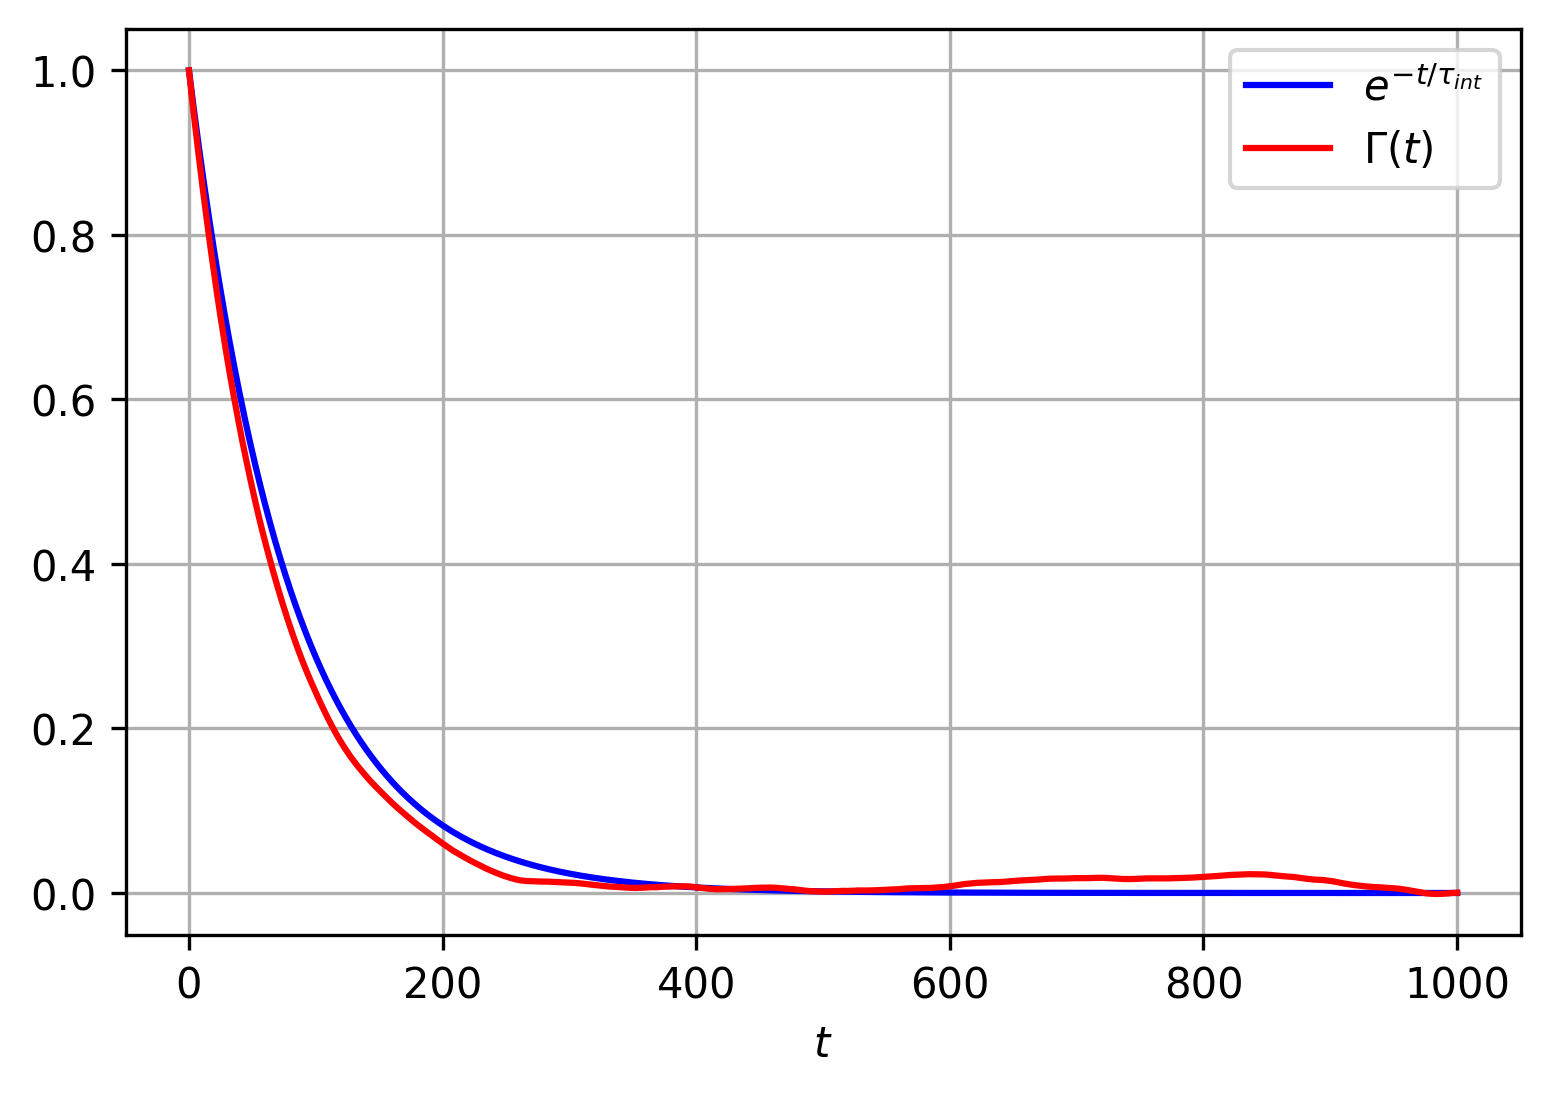
\includegraphics[scale = 0.8]{images/corr_v_e.png}
    %\caption{A plot comparing the }
    \label{fig:autocorr}
\end{figure}
\section{Autocorrelation and Bin width}
\begin{figure}[H]
    \centering
    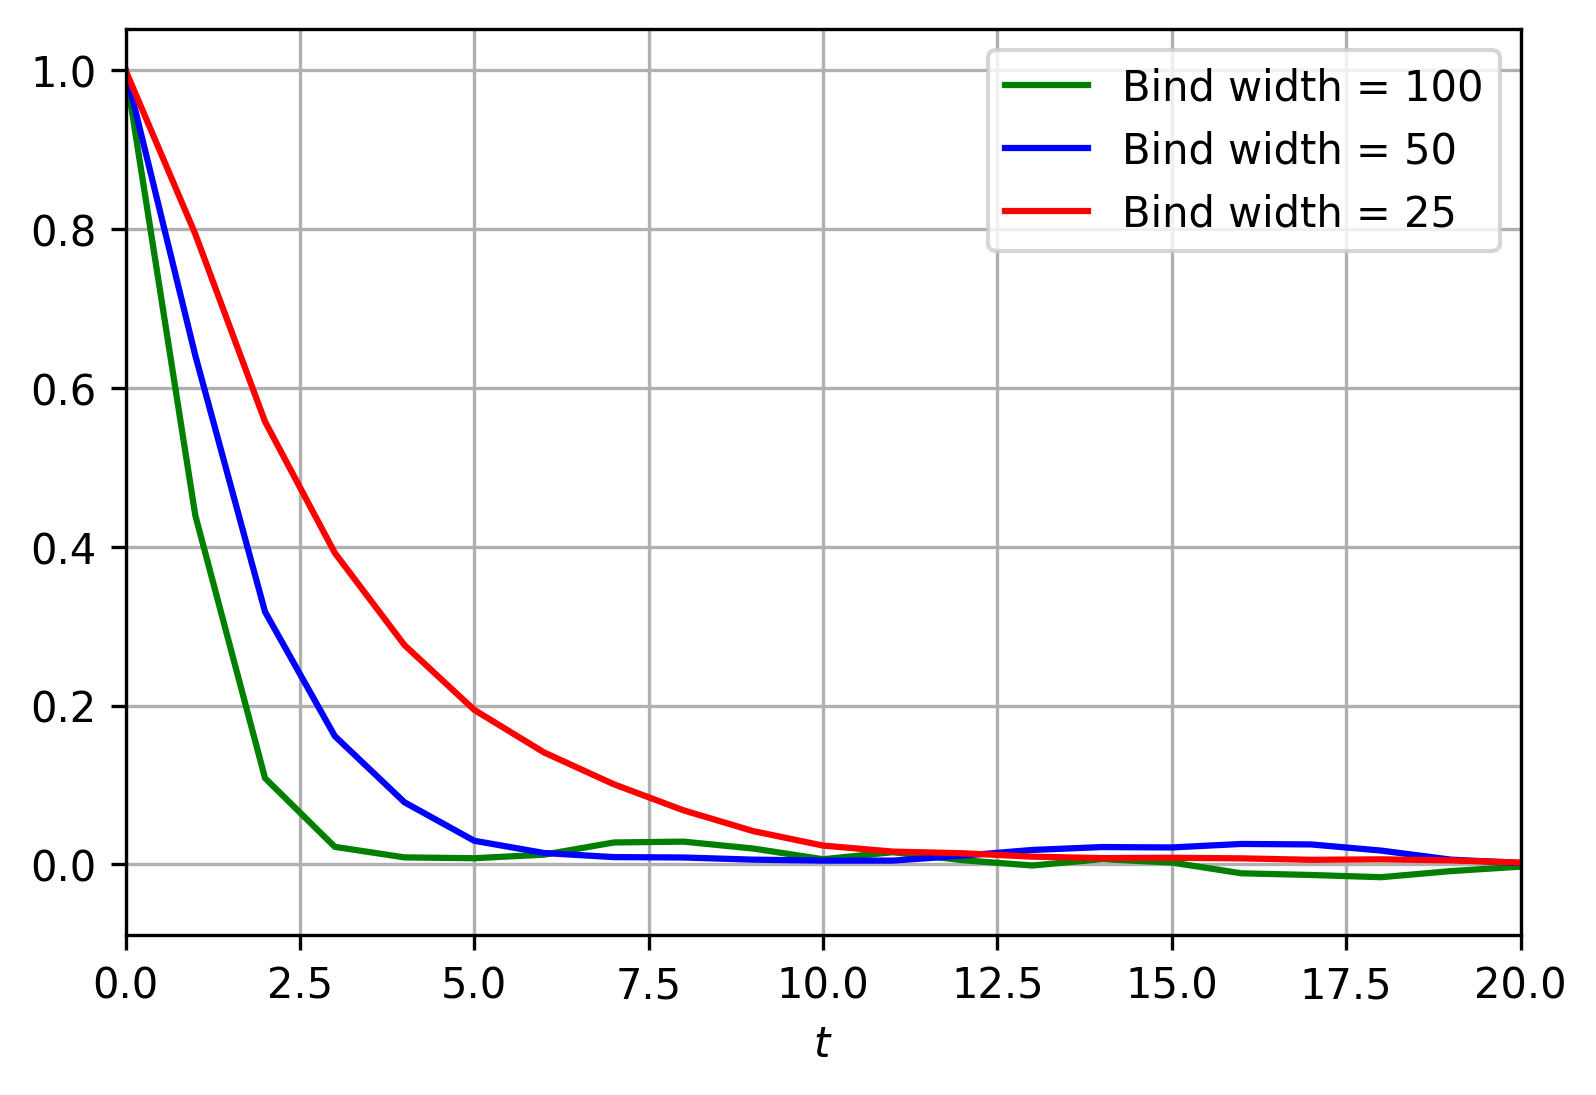
\includegraphics[scale = 0.8]{images/bin_v_t.png}
    \caption{We can see that autocorrelation decreases as the bin width is increased.. Comparing this to figure \ref{fig:autocorr}, we can also see integrated autocorrelation time has has decreased by at least a factor of 10}
    \label{fig:}
\end{figure}
\section{Behavior of the error as a function of bin width}
\begin{figure}[H]
    \centering
    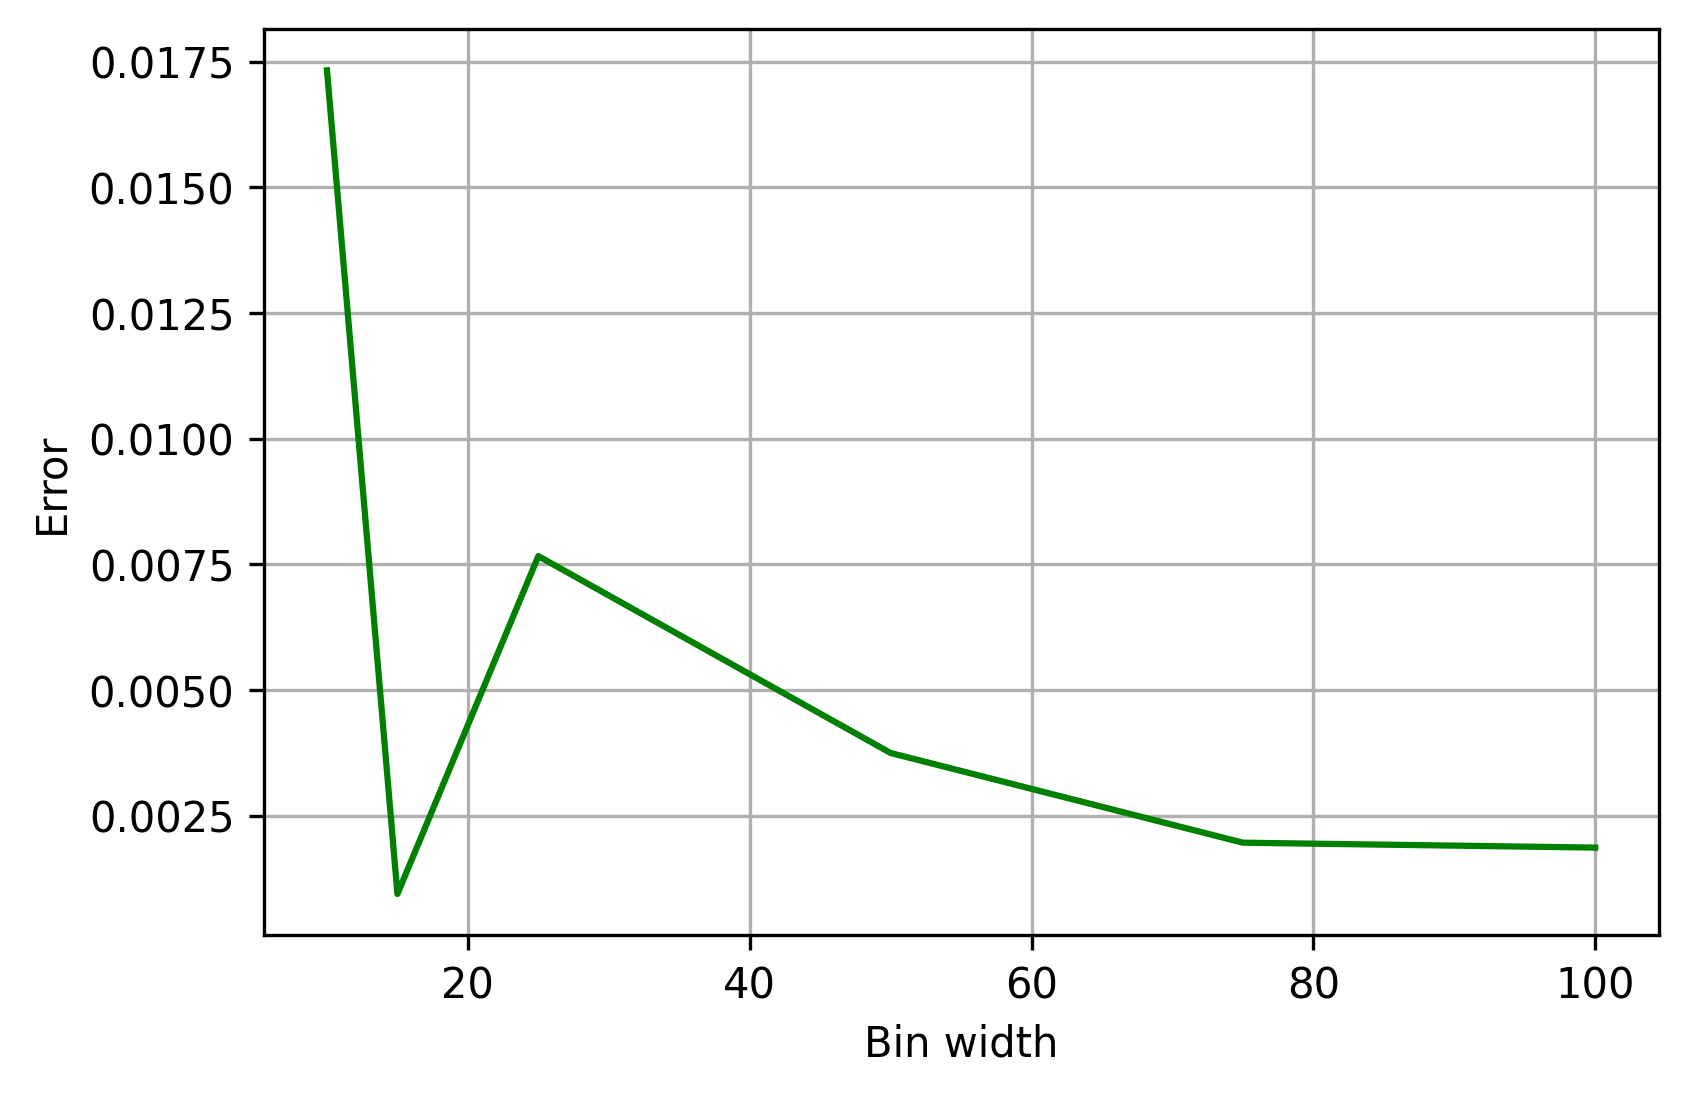
\includegraphics[scale = 0.7]{images/error_v_bin.png}
    %\caption{Caption}
    \label{fig:}
\end{figure}
\section{Error as a function of the ensemble size}
We choose a bin width of 75.
\begin{figure}[H]
    \centering
    \includegraphics[scale = 0.7]{}
    \caption{Caption}
    \label{fig:}
\end{figure}
\bibliographystyle{abbrv}
\bibliography{Bibliography.bib}
\end{document}